\documentclass[11pt]{article}

\usepackage[margin=1in]{geometry}
\usepackage{amsmath,amssymb}
\usepackage{graphicx}
\usepackage[dvipsnames,table]{xcolor}
\usepackage[round,authoryear]{natbib}
\usepackage{hyperref}
\usepackage{booktabs}
\usepackage{siunitx}

\hypersetup{colorlinks=true,linkcolor=MidnightBlue,citecolor=MidnightBlue,urlcolor=NavyBlue}

\graphicspath{{figures/}}

\newcommand{\epsnu}{\varepsilon_\nu}
\newcommand{\taua}{\tau_A}
\newcommand{\kperp}{k_\perp}
\newcommand{\zpm}{z^{\pm}}
\newcommand{\vth}{v_{\mathrm{th}}}

\title{A dissipative anomaly in the Hermite cascade of driven kinetic reduced MHD turbulence}
\author{Anjor Kanekar\\
\small Independent Researcher\\
\small \texttt{anjor@platypustech.xyz}}
\date{\today}

\begin{document}
\maketitle

\begin{abstract}
We report direct numerical evidence for a dissipative anomaly in the phase-space cascade of driven kinetic reduced magnetohydrodynamic (KRMHD) turbulence. Six simulations at $128^3$ spatial and $M=128$ Hermite resolution, driven by Alfv\'enic forcing plus a low-$\kperp$ Hermite source, were run for $200\,\taua$ each across $\nu \in \{1, 3, 5, 10, 20, 50\}$ --- a $50\times$ range in collisionality. The time-averaged collisional dissipation rate $\bar\epsnu = 49.09 \pm 0.30$ is independent of $\nu$ to better than $1\%$, while the Hermite spectrum $\langle W(m)\rangle_t$ follows the Zocco--Schekochihin $m^{-1/2}$ phase-mixing prediction in the inertial range $m \in [4, 40]$ (measured slopes $-0.472$ to $-0.496$). At the dissipation scales, $W(m)$ and $\nu$ self-adjust so that the compensated quantity $2\nu(m/M)^6 W(m)$ remains nearly invariant, with cumulative dissipation matching to $< 2\%$ across the scan. A three-point Hermite-resolution check at $\nu = 3$ over $M \in \{64, 128, 256\}$ shows the plateau value is independent of the truncation to within $\sim 2.5\%$. The result confirms the phase-space analogue of the classical hydrodynamic dissipative anomaly and establishes a direct nonlinear benchmark for KRMHD solvers.

Reaching this regime required resolving a numerical instability in the default Lawson-RK4 Hermite integrator at large $M \cdot k_z$. The fix --- an ARS(2,2,2) IMEX-RK222 scheme with implicit streaming and damping --- is described in Appendix~A and ships in GANDALF v0.5.0.
\end{abstract}

\section{Introduction}

The classical dissipative anomaly in hydrodynamic turbulence is the statement that the mean energy dissipation rate $\varepsilon$ remains finite as the viscosity $\nu \to 0$, at fixed injection. This was conjectured by \citet{onsager1949} and is a central empirical fact of high-Reynolds-number turbulence \citep{duchon2000}. The anomaly exists because the turbulent cascade delivers energy to progressively smaller scales at a rate that self-adjusts so the flux through any intermediate scale is $\nu$-independent; the dissipation scale itself moves with $\nu$, but the net dissipation does not.

The same logic ought to apply to any system that has a cascade and a dissipation mechanism acting at the far end of that cascade. In weakly collisional plasmas, KRMHD \citep{schekochihin2009} predicts a phase-space cascade in which the perturbed distribution function, expanded in Hermite moments $g_m$ of the parallel velocity, transfers energy from low $m$ to high $m$ under parallel streaming. Collisions act as a dissipation mechanism concentrated at high $m$. The obvious question is whether $\epsnu$, the collisional dissipation rate computed from the Hermite spectrum, approaches a $\nu$-independent plateau as $\nu \to 0$.

Linear phase mixing, in which $g_m$ cascades deterministically under the streaming operator alone, was analysed by \citet{zocco2011} and gives a Hermite spectrum $W(m) \propto m^{-1/2}$. The nonlinear problem, in which turbulent Alfv\'enic fluctuations at $\zpm$ nonlinearly couple to $g_m$ through the Poisson bracket $\{\Phi, g_m\}$, is much harder and has been a standing target since \citet{kanekar2015}.

The phase-space cascade has since been studied along several complementary lines. \citet{schekochihin2016} developed a scaling theory contrasting phase mixing with nonlinear advection in drift-kinetic turbulence, arguing that nonlinear coupling suppresses the leakage of free energy to high $m$ and that the energetically dominant scales are essentially fluid-like. \citet{adkins2018} solved a stochastic-electric-field model in 1D Vlasov--Hermite phase space exactly and predicted $W(m) \propto m^{-3/2}$ once anti-phase-mixing echoes dominate the nonlinear transfer. \citet{meyrand2019} reported the first nonlinear driven 3D KRMHD turbulence simulation and confirmed the fluidization picture, but at a single $\nu$ and single $M$; no $\nu$ scan and no direct test of $\bar\epsnu(\nu)$ was performed. On the theory side, \citet{eyink2018} established the existence of dissipative anomalies in nearly collisionless plasma turbulence from a coarse-grained Vlasov--Maxwell--Landau analysis, and \citet{nastac2024} demonstrated a phase-space entropy cascade and dissipative anomaly in driven gyrokinetic turbulence, providing a clear example of the phenomenon in a related kinetic system. What is missing --- and what this paper supplies --- is a direct numerical demonstration of a $\nu$-independent $\bar\epsnu$ in nonlinear driven KRMHD turbulence with the inertial range cleanly separated from the forcing and dissipation scales, via an explicit factor-of-$50$ scan in $\nu$ at fixed forcing, resolution, and $M$.

In this paper we present such a demonstration. At $128^3$ spatial resolution with $M=128$ Hermite moments and hyper-collisional damping $\propto (m/M)^6$, we drive Alfv\'enic turbulence to a steady state and then add a low-$\kperp$ forcing on the $g_0$ moment. After a $\sim\!25\,\taua$ fill-in transient the Hermite sector settles into a statistically stationary cascade. Scanning $\nu$ over a factor of $50$ produces $\bar\epsnu$ values that agree to $< 1\%$, with an inertial-range $W(m)$ slope within $\sim\!6\%$ of $m^{-1/2}$ across the scan ($\sim\!1.5\%$ for the least-damped runs) and a visible compensation between $W$ and $\nu$ at the damped scales. We interpret this as direct numerical evidence for the dissipative anomaly in a kinetic plasma turbulence problem.

An ancillary but practically important contribution is the diagnosis and fix of a scheme-level numerical instability that had previously prevented reaching this regime. The Lawson-RK4 integrator used by default in GANDALF composes an exact integrating factor for linear streaming with explicit RK stages on the nonlinear advection, which leaks a hidden CFL condition at large $M \cdot k_z$ into the stability envelope and triggers a simultaneous all-$m$ exponential blowup after $\mathcal{O}(100)\,\taua$. An IMEX-RK222 integrator \citep{ascher1997} that treats linear streaming and hyper-collisional damping implicitly resolves the instability; it ships in GANDALF v0.5.0 \citep{gandalf}. A brief account is given in Appendix~A.

\section{Model and numerics}
\label{sec:model}

We solve the KRMHD equations \citep{schekochihin2009} on a triply periodic domain of size $L_x = L_y = L_z = 1$ with $v_A = 1$, $\beta_i = 1$, and ion-to-electron temperature ratio $\tau = 1$. The state consists of the Elsasser fields $\zpm$, the parallel magnetic-field perturbation $B_\parallel$, and the first $M+1$ Hermite moments $g_m$ of the ion perturbed distribution function, with $M=128$. The coupling coefficient between the fluid and Hermite sectors is $\Lambda = \sqrt{5}$, obtained from the KRMHD dispersion relation at our parameters; it is essential to override the default $\Lambda = 1$ carried in Alfv\'enic-only checkpoints, which silently zeros the $g_0 \to g_1$ coupling through the $(1 - 1/\Lambda)$ prefactor.

Spatial resolution is $128^3$ with $2/3$ dealiasing. Forcing is applied in two channels. The Alfv\'enic drive is a balanced Elsasser white-noise forcing restricted to $n_\perp \in [1,2]$ and $|n_z| = 1$ (excluding $n_z = 0$), with amplitude $f = 0.02$, following the low-$k_z$ restriction necessary to avoid RMHD-incompatible high-$k_z$ injection. The Hermite drive acts on the $g_0$ moment only, with the same perpendicular and parallel wavenumber mask as the Alfv\'enic drive and amplitude $f_H = 3.5 \times 10^{-3}$. Resistive damping is $\eta = 100$ with hyper-order $r = 2$; Hermite damping is hyper-collisional, $\nu_m = \nu(m/M)^6$, active for $m \geq 2$.

Collisional dissipation is computed from the Hermite spectrum as
\begin{equation}
\epsnu(t) = 2\nu \sum_{m=2}^{M} \left(\frac{m}{M}\right)^6 W(m, t), \qquad W(m, t) = \sum_{\mathbf{k}} |g_m(\mathbf{k}, t)|^2.
\label{eq:eps_nu}
\end{equation}
The time-series average $\bar\epsnu$ is taken over $t - t_0 > 30\,\taua$ to exclude the Hermite fill-in transient, where $t_0$ is the time at which $g_0$ forcing is activated; the time-averaged Hermite spectra $\langle W(m)\rangle_t$ are taken over the spectrum-output window $t \in [2100, 2200]\,\taua$ (i.e.\ $t - t_0 > 100\,\taua$).

Time integration uses the IMEX-RK222 scheme of \citet{ascher1997} as implemented in GANDALF v0.5.0 \citep{gandalf}. Linear streaming and hyper-collisional damping are solved implicitly via a per-$k_z$ batched LU factorisation on the Hermite axis; the Poisson-bracket nonlinearities remain explicit. The Elsasser subsystem is advanced by an integrating-factor RK2 midpoint rule that is bit-identical to the prior Lawson-RK4 path. The timestep $\mathrm{d}t = 2.34 \times 10^{-3}$ is set by the perpendicular advection CFL with safety $0.3$. We verify the solver by running a linear Hermite benchmark with no Alfv\'enic forcing: at $M=128$, $\nu = 1$, the predicted $m^{-1/2}$ phase-mixing spectrum develops over $500\,\taua$ with $\bar\epsnu \approx 0.23$, consistent with \citet{zocco2011}.

All nonlinear runs resume from a common Alfv\'enic steady-state checkpoint at $t_0 = 2000\,\taua$, obtained by driving a pure $M = 0$ RMHD run to an $8\%$-variation steady state under the same forcing and damping. Each run extends for $200\,\taua$ of new simulated time, with $g_0$ forcing activated at $t_0$. Diagnostics are saved every $100$ steps; Hermite spectra are saved every $500$ steps during the averaging window $t \in [2100, 2200]\,\taua$.

\section{Results}
\label{sec:results}

\subsection{The \texorpdfstring{$\epsnu(\nu)$}{eps\_nu(nu)} plateau}

Figure~\ref{fig:plateau} shows the time-averaged collisional dissipation $\bar\epsnu$ as a function of $\nu$ across six runs. The six values (Table~\ref{tab:scan}) cluster at $\bar\epsnu = 49.09 \pm 0.30$; the full range is $48.42$ to $49.26$, spanning $< 2\%$. Across a factor of $50$ in $\nu$ there is no systematic trend: the plateau is flat. The spectrum-window mean (red diamonds in Figure~\ref{fig:plateau}, left panel) agrees with the full time-series mean to $\lesssim 1\%$, indicating the averaging is well converged.

\begin{table}[t]
\centering
\caption{Time-averaged dissipation, total Hermite energy, and inertial-range slope for the six IMEX runs. Time-series mean and spectrum-window mean are taken over $t - t_0 > 30\,\taua$ and $t \in [2100, 2200]\,\taua$ respectively.}
\label{tab:scan}
\begin{tabular}{cccc c}
\toprule
$\nu$ & $\bar\epsnu$ (ts) & $\bar\epsnu$ (spec) & $\langle \sum_m W(m) \rangle_t$ & slope $m \in [4, 40]$ \\
\midrule
$1$  & $48.42 \pm 11.41$ & $48.56$ & $359$ & $-0.472$ \\
$3$  & $49.21 \pm 10.65$ & $48.15$ & $162$ & $-0.484$ \\
$5$  & $49.26 \pm 10.61$ & $47.99$ & $137$ & $-0.489$ \\
$10$ & $49.23 \pm 10.81$ & $47.99$ & $126$ & $-0.493$ \\
$20$ & $49.21 \pm 10.99$ & $48.26$ & $121$ & $-0.494$ \\
$50$ & $49.21 \pm 11.21$ & $48.79$ & $114$ & $-0.496$ \\
\bottomrule
\end{tabular}
\end{table}

\begin{figure}[t]
\centering
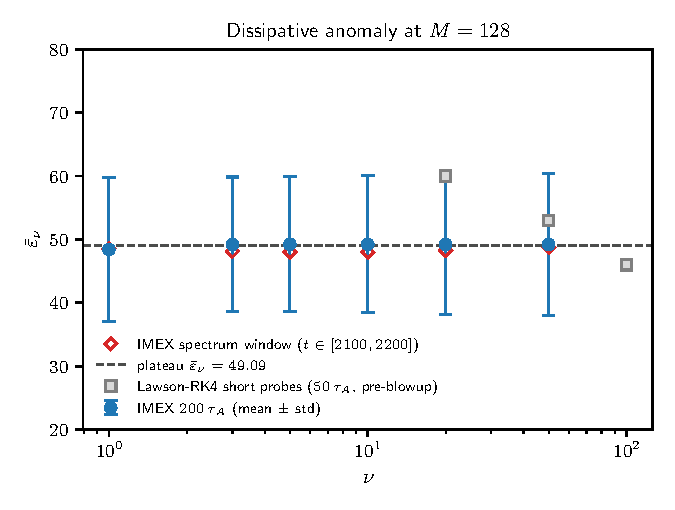
\includegraphics[width=\textwidth]{hermite128_imex_eps_nu_plateau.pdf}
\caption{\textbf{Dissipative anomaly.} Time-averaged collisional dissipation $\bar\epsnu$ as a function of $\nu$, from six IMEX runs at $M=128$, $128^3$, $200\,\taua$. Blue circles are time-series means with $\pm 1\sigma$ error bars; red diamonds are spectrum-window means. The horizontal dashed line at $\bar\epsnu = 49.09$ is the six-point mean. Gray squares are legacy Lawson-RK4 short-probe points ($50\,\taua$ before numerical blowup set in; see Appendix~A) and are shown for reference only. Across a factor of $50$ in $\nu$, $\bar\epsnu$ is flat to better than $1\%$.}
\label{fig:plateau}
\end{figure}

The corresponding self-adjustment of the spectrum at the dissipation scales is evident in Table~\ref{tab:scan}: as $\nu$ decreases, the total time-averaged Hermite energy $\langle \sum_m W(m) \rangle_t$ rises monotonically from $114$ at $\nu = 50$ to $359$ at $\nu = 1$ --- a factor of $\sim 3$ --- while $\bar\epsnu$ stays fixed. The detailed redistribution of energy in $m$ that produces this compensation is the subject of \S\ref{sec:results}.2.

\subsection{The Hermite spectrum and compensated integrand}

Figure~\ref{fig:wm} shows the time-averaged Hermite spectrum $\langle W(m) \rangle_t$ on the left and the per-$m$ dissipation integrand $2\nu(m/M)^6 W(m)$ on the right, for all six runs. The inertial range $m \in [4, 40]$ is essentially degenerate across $\nu$ on the left panel, and a log-log fit in that range returns slopes $-0.472$ (at $\nu=1$) to $-0.496$ (at $\nu=50$), with the outermost three values at $\nu = 10, 20, 50$ within $\sim\!1.5\%$ of the Zocco--Schekochihin $m^{-1/2}$ prediction. The dashed black reference line in the figure is $m^{-1/2}$ anchored at the $\nu=3$ curve.

\begin{figure}[t]
\centering
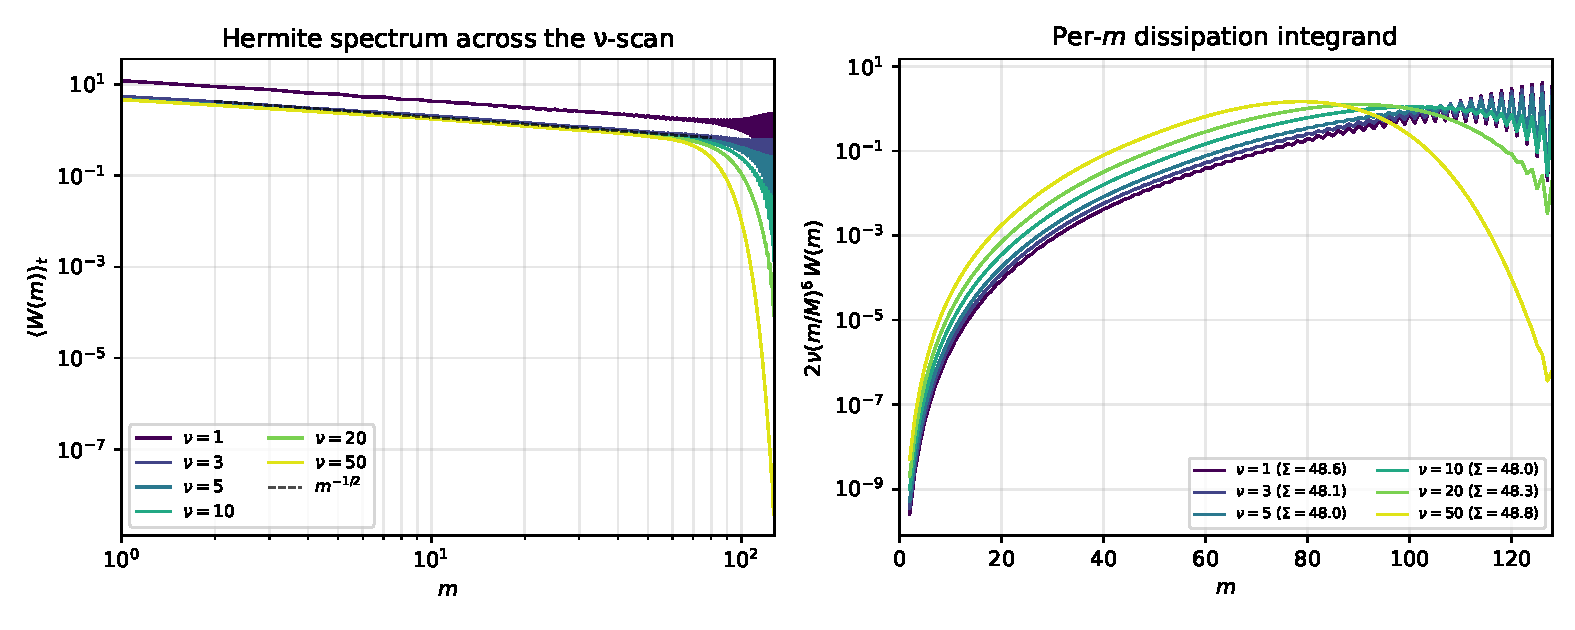
\includegraphics[width=\textwidth]{hermite128_imex_Wm_spectrum_full.pdf}
\caption{\textbf{Hermite spectrum and compensated dissipation integrand.} Left: time-averaged $\langle W(m) \rangle_t$ across the six runs, log-log, over the averaging window $t - t_0 > 100\,\taua$. Colours run from $\nu = 1$ (purple) to $\nu = 50$ (yellow). The black dashed line is the Zocco--Schekochihin prediction $W(m) \propto m^{-1/2}$. Inertial-range slopes $m \in [4, 40]$ are within $6\%$ of this line across the scan. Right: per-$m$ dissipation integrand $2\nu(m/M)^6 W(m)$. The peak shifts from near $m = M$ at low $\nu$ to $m \approx 80$ at $\nu = 50$, but the area under each curve (cumulative $\epsnu$, legend values) matches to $< 2\%$.}
\label{fig:wm}
\end{figure}

At $m \gtrsim 60$ the curves split in the expected order: lower $\nu$ carries more energy in the damped tail, because weaker collisional damping lets energy pile up before the $(m/M)^6$ factor catches it. The right panel of Figure~\ref{fig:wm} shows the corresponding dissipation integrand. At $\nu = 50$ the integrand peaks at $m \approx 80$; at $\nu = 1$ it peaks near $m = M$. But the areas under all six curves are equal to $\sim 2\%$: the cumulative values are $\epsnu \in \{48.6, 48.1, 48.0, 48.0, 48.3, 48.8\}$ (ordered by increasing $\nu$). This is the dissipative anomaly at the spectral level --- the dissipation range moves with $\nu$, the spectrum within it adjusts, and the integral that matters for the energy budget remains invariant.

\subsection{Hermite-resolution convergence}
\label{sec:Mconv}

The plateau at $M = 128$ is one slice through a two-dimensional convergence question: does $\bar\epsnu$ depend on $M$, and if so, does the $\nu$-independence we have demonstrated at $M = 128$ survive that dependence? To address this we repeated the $\nu = 3$ run at $M = 64$ (for $200\,\taua$) and at $M = 256$ (for $100\,\taua$, shortened so the run fits in a single Modal session at twice the per-step cost). The results are:

\begin{center}
\begin{tabular}{cccc}
\toprule
$M$ & $\bar\epsnu$ (ts) & $\langle \sum_m W(m) \rangle_t$ & run length \\
\midrule
$64$  & $49.11 \pm 10.99$ & $144$ & $200\,\taua$ \\
$128$ & $49.21 \pm 10.65$ & $162$ & $200\,\taua$ \\
$256$ & $50.28 \pm \phantom{0}9.92$  & $198$ & $100\,\taua$ \\
\bottomrule
\end{tabular}
\end{center}

Across a factor of $4$ in $M$, $\bar\epsnu$ shifts by $\sim 2.4\%$ --- well inside the $\pm 1\sigma$ scatter of any single time-series mean and an order of magnitude smaller than the variations one would naively expect if dissipation were limited by the truncation rather than by the cascade. The total Hermite energy $\langle \sum_m W(m) \rangle_t$ does grow monotonically with $M$ (from $144$ at $M = 64$ to $198$ at $M = 256$), as expected: increasing $M$ moves the hyper-collisional cutoff $\nu(m/M)^6$ outward in $m$ and the cascade fills the extra room before being damped. The dissipation rate, which is the integral that matters for the energy budget, is unaffected. This is the $M$-convergence content of the dissipative anomaly: not only is $\bar\epsnu$ independent of $\nu$ at fixed $M$, it is also independent of $M$ at fixed $\nu$, at this resolution.

Figure~\ref{fig:basestate} documents the base state and the absence of a Hermite pileup, for the $\nu = 3$ run. The left panel is the time-averaged perpendicular energy spectrum $E(\kperp)$ of the driven state: a forced band at $\kperp \lesssim 12$, a short inertial range consistent with $\kperp^{-3/2}$, and a clean resistive cutoff beyond $\kperp \approx 40$. The base state is a legitimate, if modest, Alfv\'enic cascade and not a pathological or under-resolved one. The right panel is the Hermite spectrum $W(m, t)$ over the stationary window: the energy stays concentrated at low $m$ and decays monotonically to a tail at $m = M$ carrying only $\sim 2\%$ of the $m = 0$ value, with no growth over the $100\,\taua$ shown. There is no pileup at the truncation and no blowup --- in contrast to the Lawson-RK4 behaviour of Appendix~A.

\begin{figure}[t]
\centering
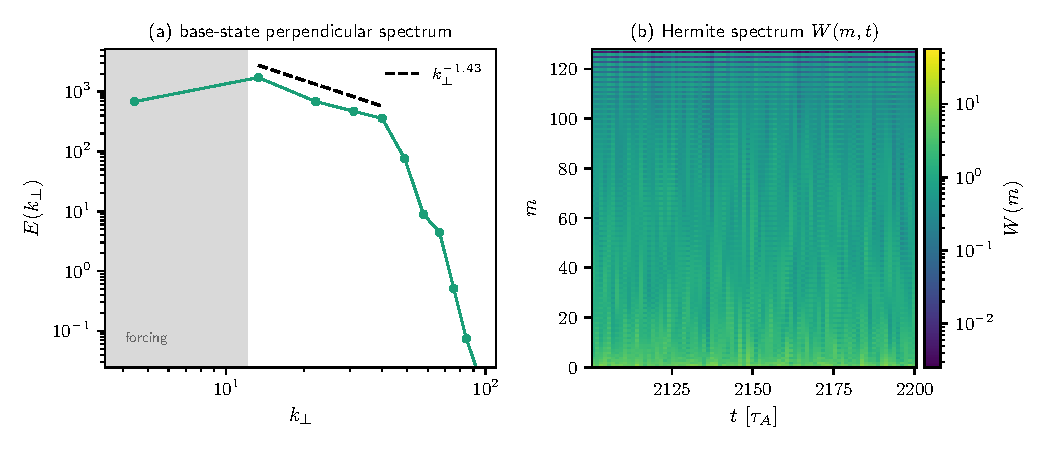
\includegraphics[width=\textwidth]{hermite128_nu3_imex_basestate_wmt.pdf}
\caption{\textbf{Base state and absence of a Hermite pileup}, from the $\nu = 3$ IMEX run. Left: time-averaged perpendicular energy spectrum $E(\kperp)$ over $t \in [2100, 2200]\,\taua$. The shaded band is the forcing range; the dashed line is the measured inertial-range slope $\kperp^{-1.43}$, close to $\kperp^{-3/2}$, fitted over $\kperp \in [12, 42]$. The steep fall beyond is the hyper-resistive cutoff. Right: Hermite spectrum $W(m, t)$ over the same window. Energy remains concentrated at low $m$ and stationary in time; the $m = M$ tail is $\sim 2\%$ of the $m = 0$ peak and does not grow. The horizontal banding at high $m$ is the even/odd Hermite parity of the streaming operator.}
\label{fig:basestate}
\end{figure}

\section{Discussion}
\label{sec:discussion}

The plateau in $\bar\epsnu(\nu)$ is the standard signature of a constant-flux turbulent cascade. A driven turbulence problem separates into three scale ranges: a forcing range, an inertial range, and a dissipation range. In the inertial range, energy is transferred between scales without being removed, so the flux through any intermediate scale is constant in scale --- it is set by the inertial-range dynamics, not by the dissipation mechanism. As $\nu$ decreases, the dissipation range retreats to higher $m$, but the inertial-range flux is unchanged. The integrated collisional dissipation $\bar\epsnu$, which is whatever the inertial range delivers to the damped scales, therefore approaches a $\nu$-independent value. The flat plateau across our factor-of-$50$ scan is the integrated form of this statement; the moment-space redistribution of energy that supports it is shown directly in Figure~\ref{fig:wm}.

The crossover at $\nu \approx 3$, visible as a kink in the total Hermite energy reported in Table~\ref{tab:scan}, is naturally interpreted in this picture. At large $\nu$, the hyper-collisional damping $\nu(m/M)^6$ is broad enough to reach into the nominal inertial range; modes in $m \in [4, 40]$ partially feel the dissipation and the inertial range is short. As $\nu$ decreases, the dissipation range retreats to higher $m$ and the inertial range becomes oblivious to $\nu$, in the sense that $W(m)$ in the inertial range no longer depends on $\nu$. The plateau in $\bar\epsnu$ holds across both regimes because injection still sets the dissipation rate; the constant-flux argument does not require the inertial range to be wide, only that one exists.

Two caveats delimit the result. The plateau is a finite-$\nu$, finite-$M$ statement: with the cascade truncated at $m = M$, the genuinely collisionless limit $\nu \to 0$ at fixed $M$ is not directly accessible. The $M$-convergence check in \S\ref{sec:Mconv} shows that $\bar\epsnu$ is stable to within $\sim 2.5\%$ across $M \in \{64, 128, 256\}$ at $\nu = 3$, so at this $\nu$ the plateau value is set by the cascade rather than by the truncation, but we cannot extrapolate to arbitrarily small $\nu$ without further $M$-scans at the low-$\nu$ end of the scan, where the cascade reaches further into $m$. Second, the perpendicular inertial range in our $128^3$ setup is short (Figure~\ref{fig:basestate}); a larger $k_\perp$ dynamic range would strengthen the constant-flux argument on the perpendicular side and would let us probe the regime where echoes from imbalanced cascades could matter.

Our nonlinear simulations reproduce the linear phase-mixing slope $W(m) \propto m^{-1/2}$ of \citet{zocco2011} to within $6\%$ across the scan, and to within $\sim\!1.5\%$ for the three least-damped runs. The \citet{adkins2018} solvable model of stochastic phase mixing predicts a steeper $m^{-3/2}$ scaling once anti-phase-mixing echoes dominate the nonlinear transfer; we do not see that scaling at our resolution. Whether the absence reflects a fundamental feature of KRMHD turbulence at our parameters --- balanced, weakly compressible, $\beta_i = 1$ --- or simply insufficient dynamic range in $m$ and $\kperp$ remains open. Extending the \citet{meyrand2019} fluidization picture to imbalanced turbulence, where the echo mechanism is expected to be progressively suppressed by cross-helicity, is a separate direction we are pursuing in follow-up work.

\section*{Acknowledgements}

Compute for the simulations reported here was provided by Modal. The author thanks A.~A. Schekochihin for discussions of the phase-space cascade and its connection to the dissipative anomaly. This work was carried out with assistance from Claude (Anthropic), including the development and code review of the GANDALF v0.5.0 IMEX-RK222 integrator; the author takes full responsibility for all scientific content.

\appendix

\section{A numerical instability in Lawson-RK4 and the IMEX-RK222 fix}
\label{app:imex}

Every nonlinear Hermite run attempted with GANDALF's default Lawson-RK4 integrator blew up. The onset was delayed, but not prevented, by collisionality: it set in at $\approx 80\,\taua$ for $\nu = 1$, $122\,\taua$ for $\nu = 3$, $167\,\taua$ for $\nu = 5$, and $184\,\taua$ for $\nu = 10$. The monotonic dependence of the onset time on $\nu$ initially suggested a physical pileup of energy at the truncation.

Three diagnostics ruled that out. First, $W(m = M)$ remained bounded at the $\mathcal{O}(1)$ noise level until the moment of blowup, with no gradual accumulation beforehand. Second, the parallel-wavenumber spectrum of $g_m$ at $m = M$ sat at the $10^{-14}$ floor throughout --- no flux was reaching the truncation. Third, when the blowup occurred, all Hermite moments grew exponentially at once, at a $\nu$-independent rate; a physical cascade pileup would instead localise in $m$. Together these signatures identify a scheme-level stability failure rather than a physical cascade overflow.

The mechanism lies in the Lawson composition. Lawson-RK4 applies an exact integrating factor $\exp(\mathcal{L}_{\mathrm{stream}}\,\mathrm{d}t)$ for the linear streaming operator and explicit Runge--Kutta stages for the Poisson-bracket nonlinearity. For pure streaming this is exact and norm-preserving, but composing it with the explicit stages leaks a hidden CFL condition, $\mathrm{d}t\,\vth\,k_z\sqrt{m}/\Lambda$, into the stability envelope. At $M = 128$, $128^3$, with low-$k_z$ forcing and a CFL safety factor of $0.3$, this quantity is $\mathcal{O}(1)$ and the scheme is marginally unstable --- enough to seed a slow exponential growth that eventually dominates.

The fix is the ARS(2,2,2) IMEX-RK222 scheme of \citet{ascher1997}: the linear streaming and hyper-collisional damping are treated implicitly via a per-$k_z$ tridiagonal LU factorisation on the Hermite axis, while the nonlinear advection remains explicit. This removes the linear terms from the explicit stability constraint, which is then set by the standard perpendicular-advection CFL alone. The scheme ships in GANDALF v0.5.0 (pull request \#138); its acceptance test --- $\nu = 3$, $M = 128$, $128^3$, $200\,\taua$ --- cleared on the first attempt. Detailed diagnostic figures and the supporting analysis are archived with the run records (\texttt{docs/hermite\_handoff.md} and \texttt{analysis/diagnose\_hermite\_blowup.py}).

\bibliographystyle{plainnat}
\bibliography{refs}

\end{document}
